\documentclass[tikz,border=10pt]{standalone}
\usepackage{tikz}
\usepackage{amsmath}
\usetikzlibrary{arrows.meta}

\begin{document}

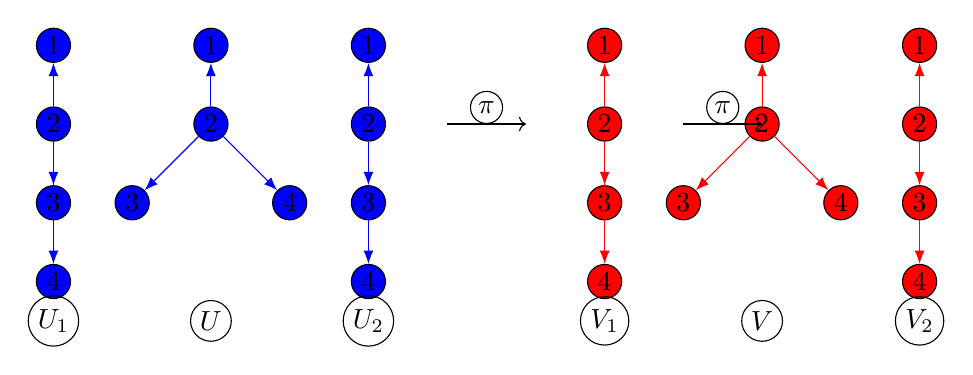
\begin{tikzpicture}[every node/.style={circle, draw, inner sep=1.5pt},
                    every path/.style={-Latex}]

    % First Tree
    \node[fill=blue] (a1) at (0,1) {1};
    \node[fill=blue] (a2) at (0,0) {2};
    \node[fill=blue] (a3) at (0,-1) {3};
    \node[fill=blue] (a4) at (0,-2) {4};
    
    \node at (0,-2.5) {$U_1$};
    
    \draw[blue] (a2) -- (a1);
    \draw[blue] (a2) -- (a3);
    \draw[blue] (a2) -- (a4);

    % Second Tree
    \node[fill=blue] (b1) at (2,1) {1};
    \node[fill=blue] (b2) at (2,0) {2};
    \node[fill=blue] (b3) at (1,-1) {3};
    \node[fill=blue] (b4) at (3,-1) {4};
    
    \node at (2,-2.5) {$U$};
    
    \draw[blue] (b2) -- (b1);
    \draw[blue] (b2) -- (b3);
    \draw[blue] (b2) -- (b4);

    % Third Tree
    \node[fill=blue] (c1) at (4,1) {1};
    \node[fill=blue] (c2) at (4,0) {2};
    \node[fill=blue] (c3) at (4,-1) {3};
    \node[fill=blue] (c4) at (4,-2) {4};
    
    \node at (4,-2.5) {$U_2$};
    
    \draw[blue] (c2) -- (c1);
    \draw[blue] (c3) -- (c4);
    \draw[blue] (c2) -- (c3);

    % Arrow for first transformation
    \draw[->] (5,0) -- node[midway, above] {$\pi$} (6,0);

    % Fourth Tree
    \node[fill=red] (d1) at (7,1) {1};
    \node[fill=red] (d2) at (7,0) {2};
    \node[fill=red] (d3) at (7,-1) {3};
    \node[fill=red] (d4) at (7,-2) {4};
    
    \node at (7,-2.5) {$V_1$};
    
    \draw[red] (d2) -- (d1);
    \draw[red] (d2) -- (d3);
    \draw[red] (d2) -- (d4);

    % Fifth Tree
    \node[fill=red] (e1) at (9,1) {1};
    \node[fill=red] (e2) at (9,0) {2};
    \node[fill=red] (e3) at (8,-1) {3};
    \node[fill=red] (e4) at (10,-1) {4};
    
    \node at (9,-2.5) {$V$};
    
    \draw[red] (e2) -- (e1);
    \draw[red] (e2) -- (e3);
    \draw[red] (e2) -- (e4);

    % Sixth Tree
    \node[fill=red] (f1) at (11,1) {1};
    \node[fill=red] (f2) at (11,0) {2};
    \node[fill=red] (f3) at (11,-1) {3};
    \node[fill=red] (f4) at (11,-2) {4};
    
    \node at (11,-2.5) {$V_2$};
    
    \draw[red] (f2) -- (f1);
    \draw[red] (f3) -- (f4);
    \draw[red] (f2) -- (f3);

    % Arrow for second transformation
    \draw[->] (8,0) -- node[midway, above] {$\pi$} (9,0);

\end{tikzpicture}

\end{document}